%!TEX root = PMP_ClockPendulumAnalyzer.tex
\subsection*{Sprint 1}
Die Planung und der Abschluss von Sprint 1 ist in diesem Kapitel aufgeführt.
\subsubsection*{Planung}
Die Planung der Sprints wurde mit dem Programm Taiga.io durchgeführt. Unten ist ein Screenshot zu Beginn von Sprint 1.
    \begin{figure}[H]
        \centering
        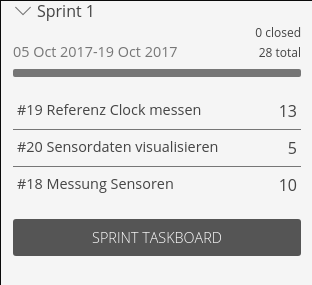
\includegraphics[width=.5\textwidth]{sprint1_plan.png}
        \caption{Sprintplanung für Sprint 1}
    \end{figure}
\subsubsection*{Sprintreview}
    Sprint 1 wurde mit zufrieden stellenden Ergebnissen aus verschiedenen einzelnen Tasks beendet. Die involvierten User Stories wurden mit untenstehender Begründung in den nächsten Sprint verschoben.
    \begin{table}[H]
        \centering
        \begin{tabular}{lccp{7cm}}
            \textbf{User Story} &  \textbf{Status} & \textbf{Sprintziel}& \textbf{Begründung}\\\toprule[2pt]
            \#19 Referenz Clock messen & teilweise erledigt & Verschoben & Auf Grund von Wartezeiten\\
            \#20 Sensordaten visualisieren & teilweise erledigt & Verschoben & einzelne Tasks konnten wegen fehlendem Werkzeug nicht komplettiert werden\\
            \#18 Messung Sensoren & teilweise erledigt & Verschoben & Tasks konnten aufgrund Abwesenheit nicht vervollständigt werden\\
        \end{tabular}
        \caption{Status der User Stories aus Sprint 1}
    \end{table}

\clearpage
\subsection*{Sprint 2}
Die Planung und der Abschluss von Sprint 2 ist in diesem Kapitel aufgeführt.
\subsubsection*{Planung}
Der Sprint enthält die gleichen User Stories wie der 1. Sprint, weil alle Pakete in diesen Sprint verschoben wurden.
\begin{figure}[H]
    \centering
    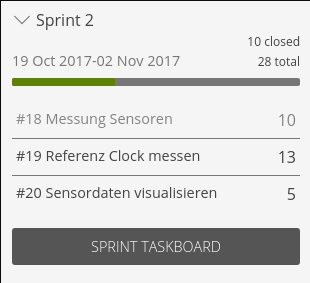
\includegraphics[width=.5\textwidth]{sprint2_plan.png}
    \caption{Sprintplanung für Sprint 2}
\end{figure}
\subsubsection*{Sprintreview}
Aufgrund von zu wenig Wissen über Hardware und Sensorik war der Fortschritt nur schwerfällig. Mit Hilfe eines Logic Analyzer (LA) konnte die RTC und der Sensor überprüft werden. Daraus ergab sich, dass der Sensor neu gelötet werden muss. Die RTC war in Ordnung. Der Zugriff auf die GPIO wurde ebenfalls umgesetzt. Somit wurden alle Sprintziele erreicht
\begin{table}[H]
    \centering
    \begin{tabular}{lccp{7cm}}
        \textbf{User Story} &  \textbf{Status} & \textbf{Sprintziel}& \textbf{Begründung}\\\toprule[2pt]
        \#19 Referenz Clock messen & erledigt & erreicht & mit LA gemessen\\
        \#20 Sensordaten visualisieren & erledigt & erreicht & Sensor und GPIO wurden korrekt in Betrieb genommen\\
        \#18 Messung Sensoren & erledigt & erreicht & LA gab auf Sensor nichts aus dafür aber der provisorische Python Zugriff\\
    \end{tabular}
    \caption{Status der User Stories aus Sprint 2}
\end{table}

\clearpage
\subsection*{Sprint 3}
Die Planung und der Abschluss von Sprint 3 ist in diesem Kapitel aufgeführt.
\subsubsection*{Planung}
Sprint 3 enthält eine grosse User Story für das Entwerfen und Erstellen eines PCB mit einem Hardware Counter. Dazu wird noch die Datenpersistenz entwickelt.
\begin{figure}[H]
    \centering
    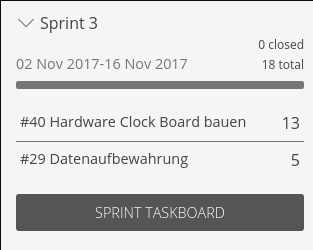
\includegraphics[width=.5\textwidth]{sprint3_plan.png}
    \caption{Sprintplanung für Sprint 3}
\end{figure}
\subsubsection*{Sprintreview}
Da es für die Entwicklung eines Schemas und Layouts für PCBs das Wissen braucht, wie die einzelnen Komponenten angeschlossen werden, konnte die UserStory für das erstellen eines Counterboards nicht fertig gestellt werden. Dafür wurde bereits ein Teil der Software entwickelt zum Ansteuern und die einzelnen Komponenten in Betrieb genommen.\\
Aufgrund einer schlechten Zuständigkeitsverteilung wurde die 2. UserStory ebenfalls nicht fertiggestellt. Deshalb werden diese nun auf den nächsten Sprint verschoben.
\begin{table}[H]
    \centering
    \begin{tabular}{p{4cm}ccp{7cm}}
        \textbf{User Story} &  \textbf{Status} & \textbf{Sprintziel}& \textbf{Begründung}\\\toprule[2pt]
        \#40 Hardware Clock Board bauen & teilweise erledigt & Verschoben & Zu wenig Vorkenntnisse über die Ansteuerung der einzelnen Komponenten\\
        \#29 Datenaufbewahrung & teilweise erledigt & Verschoben & Zuständigkeiten wurden schlecht verteilt und somit zu spät mit der Realisierung begonnen\\
    \end{tabular}
    \caption{Status der User Stories aus Sprint 3}
\end{table}

\clearpage
\subsection*{Sprint 4}
Die Planung und der Abschluss von Sprint 4 ist in diesem Kapitel aufgeführt.
\subsubsection*{Planung}
Im Sprint 4 werden die UserStories aus Sprint 3 weitergeführt, die nicht beendet worden sind. Da einige Tasks in den Stories von Sprint 3 erledigt sind wird noch die User Story für die Visualisierung eingesetzt. Diese bekommt die kleinste Priorität.
\begin{figure}[H]
    \centering
    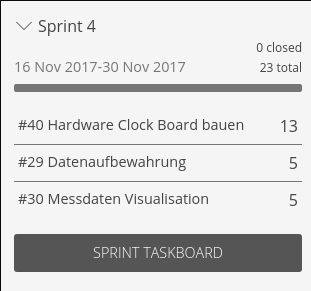
\includegraphics[width=.5\textwidth]{sprint4_plan.png}
    \caption{Sprintplanung für Sprint 4}
\end{figure}

\subsubsection*{Sprintreview}
Die grösste UserStory für das Entwickeln des Hardware Counterboard konnte beendet werden. Die Software zum Counterboard wurde einer neuen User Story zugeteilt und wird als einzelner Task behandelt.\\
Die UserStory \#29 Datenaufbewahrung wird auf den nächsten Sprint geschoben, weil mehr Entwicklungsaufwand benötigt wird. Die User Story für die Visualisierung wurde im Sprint 4 so eingeplant dass diese nur teilweise erledigt werden soll. Somit wird diese ebenfalls in Sprint 5 geschoben.
\begin{table}[H]
    \centering
    \begin{tabular}{p{4cm}ccp{7cm}}
        \textbf{User Story} &  \textbf{Status} & \textbf{Sprintziel}& \textbf{Begründung}\\\toprule[2pt]
        \#40 Hardware Clock Board bauen & erledigt & Erreicht & Board erstellt und Software in UserStory ausgelagert\\
        \#29 Datenaufbewahrung & teilweise erledigt & Verschoben & Komplexität der Gesamtsoftware braucht mehr Zeit\\
        \#30 Messdaten Visualisation & ausstehend & Verschoben & Es wurden nur Lösungsvorschläge gesucht, keine Umsetzung\\
    \end{tabular}
    \caption{Status der User Stories aus Sprint 4}
\end{table}

\clearpage
\subsection*{Sprint 5}
Die Planung und der Abschluss von Sprint 5 ist in diesem Kapitel aufgeführt.
\subsubsection*{Planung}
Im Sprint 5 sind weitere User Stories zur Software geplant. Das Entwickeln eines Client zur Visualisierung der Messergebnisse, Datenbankanbindung, Timer/Counter auf dem Hardware Counterboard sowie Schnittstelle zwischen Client und Messgerät.
\begin{figure}[H]
    \centering
    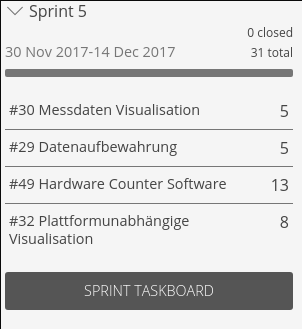
\includegraphics[width=.5\textwidth]{sprint5_plan.png}
    \caption{Sprintplanung für Sprint 5}
\end{figure}
\subsubsection*{Sprintreview}%TODO sprint 5 review
Die User Stories konnten wegen zu hoher Dokumentationsarbeit nicht weiter verfolgt werden. Die User Story für die Datenaufbewahrung konnte nebenbei komplettiert werden. Alle anderen geplanten User Stories wurden weiter verschoben und werden nun in der Testphase weiterentwickelt.\\\\
Die letzte Phase wird nicht als Sprint geplant.
\begin{table}[H]
    \centering
    \begin{tabular}{p{4cm}ccp{7cm}}
        \textbf{User Story} &  \textbf{Status} & \textbf{Sprintziel}& \textbf{Begründung}\\\toprule[2pt]
        \#29 Datenaufbewahrung & erledigt & Erreicht & Die Datenbankanbindung läuft nun\\
        \#30 Messdaten Visualisierung & ausstehend & Verschoben & Aufgrund anderer ausstehender Arbeiten wurde diese User Story weiter verschoben\\
        \#49 Hardware Counter Software & teilweise erledigt & Verschoben & Es konnten die meisten Aufgaben implementiert werden. Sie wird verschoben bis alles implementiert ist.\\
        \#32 Plattformunabhängige Visualisierung & teilweise erledigt & Verschoben & Einzelne Tasks konnten bereits umgesetzt werden.\\
    \end{tabular}
    \caption{Status der User Stories aus Sprint 5}
\end{table}